\begin{figure}[h]
    \begin{center}[h]
        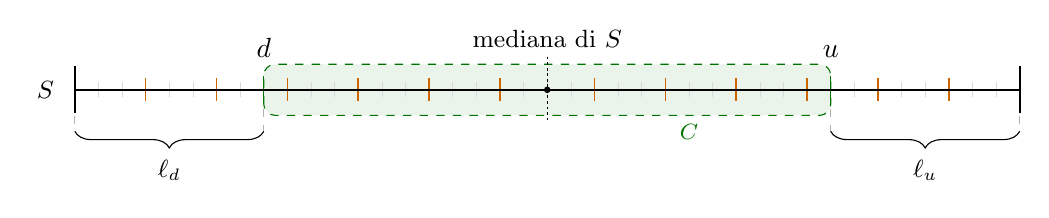
\begin{tikzpicture}[scale=1.2, every node/.style={font=\small}]
        % AREA C
        \fill[green!45!black, opacity=0.08, rounded corners=4pt] (-3, -0.27) rectangle (3, 0.27);
        \draw[green!45!black, thin, dashed, rounded corners=4pt] (-3, -0.27) rectangle (3, 0.27);
        \node[green!45!black, font=\footnotesize\bfseries] at (1.5, -0.45) {$C$};

        % ELEMENTI DI S
        \foreach \i in {1,2,...,39}
            \draw[gray!30, very thin] ({-5 + \i*(10/40)}, 0.08) -- ({-5 + \i*(10/40)}, -0.08);

        % ELEMENTI DI R 
        \foreach \i in {3, 6, 9, 12, 15, 18, 22, 25, 28, 31, 34, 37}
            \draw[orange!80!black, semithick] ({-5 + \i*(10/40)}, 0.12) -- ({-5 + \i*(10/40)}, -0.12);

        \draw[green!45!black] (-3, 0.15) -- (-3, -0.15);
        \draw[green!45!black] (3, 0.15) -- (3, -0.15);

        \node[above=8pt, font=\bfseries] at (-3,0) {$d$};
        \node[above=8pt, font=\bfseries] at (3,0) {$u$};
        \node[above=14pt, fill=white, inner sep=1pt] at (0,0) {mediana di $S$};

        \draw[gray!60, thin, dashed] (-5,-0.1) -- (-5,-0.45);
        \draw[gray!60, thin, dashed] (-3,-0.2) -- (-3,-0.45);
        \draw[gray!60, thin, dashed] (3,-0.2) -- (3,-0.45);
        \draw[gray!60, thin, dashed] (5,-0.1) -- (5,-0.45);

        \draw[decorate, decoration={brace, mirror, raise=15pt, amplitude=6pt}]
            (-5,0) -- (-3,0)
            node[midway, below=22pt] {$\ell_d$};

        \draw[decorate, decoration={brace, mirror, raise=15pt, amplitude=6pt}]
            (3,0) -- (5,0)
            node[midway, below=22pt] {$\ell_u$};

        \draw[thick] (-5,0) -- (5,0);
        \draw[thick] (-5,0.25) -- (-5,-0.25);
        \draw[thick] (5,0.25) -- (5,-0.25);
        \node[left=4pt] at (-5,0) {$S$};

        \draw[dash pattern= on 1 pt] (0, 0.35) -- (0, -0.35);
        \filldraw (0,0) circle (0.8pt);
        \end{tikzpicture}
    \end{center}
    \label{fig:2}
    \caption{Rappresentazione grafica degli insiemi usati dall'algoritmo}
\end{figure}